
%% bare_jrnl_compsoc.tex
%% V1.3
%% 2007/01/11
%% by Michael Shell
%% See:
%% http://www.michaelshell.org/
%% for current contact information.
%%
%% This is a skeleton file demonstrating the use of IEEEtran.cls
%% (requires IEEEtran.cls version 1.7 or later) with an IEEE Computer
%% Society journal paper.
%%
%% Support sites:
%% http://www.michaelshell.org/tex/ieeetran/
%% http://www.ctan.org/tex-archive/macros/latex/contrib/IEEEtran/
%% and
%% http://www.ieee.org/

%%*************************************************************************
%% Legal Notice:
%% This code is offered as-is without any warranty either expressed or
%% implied; without even the implied warranty of MERCHANTABILITY or
%% FITNESS FOR A PARTICULAR PURPOSE! 
%% User assumes all risk.
%% In no event shall IEEE or any contributor to this code be liable for
%% any damages or losses, including, but not limited to, incidental,
%% consequential, or any other damages, resulting from the use or misuse
%% of any information contained here.
%%
%% All comments are the opinions of their respective authors and are not
%% necessarily endorsed by the IEEE.
%%
%% This work is distributed under the LaTeX Project Public License (LPPL)
%% ( http://www.latex-project.org/ ) version 1.3, and may be freely used,
%% distributed and modified. A copy of the LPPL, version 1.3, is included
%% in the base LaTeX documentation of all distributions of LaTeX released
%% 2003/12/01 or later.
%% Retain all contribution notices and credits.
%% ** Modified files should be clearly indicated as such, including  **
%% ** renaming them and changing author support contact information. **
%%
%% File list of work: IEEEtran.cls, IEEEtran_HOWTO.pdf, bare_adv.tex,
%%                    bare_conf.tex, bare_jrnl.tex, bare_jrnl_compsoc.tex
%%*************************************************************************

% *** Authors should verify (and, if needed, correct) their LaTeX system  ***
% *** with the testflow diagnostic prior to trusting their LaTeX platform ***
% *** with production work. IEEE's font choices can trigger bugs that do  ***
% *** not appear when using other class files.                            ***
% The testflow support page is at:
% http://www.michaelshell.org/tex/testflow/




% Note that the a4paper option is mainly intended so that authors in
% countries using A4 can easily print to A4 and see how their papers will
% look in print - the typesetting of the document will not typically be
% affected with changes in paper size (but the bottom and side margins will).
% Use the testflow package mentioned above to verify correct handling of
% both paper sizes by the user's LaTeX system.
%
% Also note that the "draftcls" or "draftclsnofoot", not "draft", option
% should be used if it is desired that the figures are to be displayed in
% draft mode.
%
% The Computer Society usually requires 12pt for submissions.
%
\documentclass[12pt,journal,compsoc]{IEEEtran}
%
% If IEEEtran.cls has not been installed into the LaTeX system files,
% manually specify the path to it like:
% \documentclass[12pt,journal,compsoc]{../sty/IEEEtran}





% Some very useful LaTeX packages include:
% (uncomment the ones you want to load)

\usepackage{float}
\usepackage{amsmath}
\usepackage{graphicx}

% *** MISC UTILITY PACKAGES ***
%
%\usepackage{ifpdf}
% Heiko Oberdiek's ifpdf.sty is very useful if you need conditional
% compilation based on whether the output is pdf or dvi.
% usage:
% \ifpdf
%   % pdf code
% \else
%   % dvi code
% \fi
% The latest version of ifpdf.sty can be obtained from:
% http://www.ctan.org/tex-archive/macros/latex/contrib/oberdiek/
% Also, note that IEEEtran.cls V1.7 and later provides a builtin
% \ifCLASSINFOpdf conditional that works the same way.
% When switching from latex to pdflatex and vice-versa, the compiler may
% have to be run twice to clear warning/error messages.






% *** CITATION PACKAGES ***
%
\ifCLASSOPTIONcompsoc
  % IEEE Computer Society needs nocompress option
  % requires cite.sty v4.0 or later (November 2003)
  % \usepackage[nocompress]{cite}
\else
  % normal IEEE
  % \usepackage{cite}
\fi
% cite.sty was written by Donald Arseneau
% V1.6 and later of IEEEtran pre-defines the format of the cite.sty package
% \cite{} output to follow that of IEEE. Loading the cite package will
% result in citation numbers being automatically sorted and properly
% "compressed/ranged". e.g., [1], [9], [2], [7], [5], [6] without using
% cite.sty will become [1], [2], [5]--[7], [9] using cite.sty. cite.sty's
% \cite will automatically add leading space, if needed. Use cite.sty's
% noadjust option (cite.sty V3.8 and later) if you want to turn this off.
% cite.sty is already installed on most LaTeX systems. Be sure and use
% version 4.0 (2003-05-27) and later if using hyperref.sty. cite.sty does
% not currently provide for hyperlinked citations.
% The latest version can be obtained at:
% http://www.ctan.org/tex-archive/macros/latex/contrib/cite/
% The documentation is contained in the cite.sty file itself.
%
% Note that some packages require special options to format as the Computer
% Society requires. In particular, Computer Society  papers do not use
% compressed citation ranges as is done in typical IEEE papers
% (e.g., [1]-[4]). Instead, they list every citation separately in order
% (e.g., [1], [2], [3], [4]). To get the latter we need to load the cite
% package with the nocompress option which is supported by cite.sty v4.0
% and later. Note also the use of a CLASSOPTION conditional provided by
% IEEEtran.cls V1.7 and later.





% *** GRAPHICS RELATED PACKAGES ***
%
\ifCLASSINFOpdf
  % \usepackage[pdftex]{graphicx}
  % declare the path(s) where your graphic files are
  % \graphicspath{{../pdf/}{../jpeg/}}
  % and their extensions so you won't have to specify these with
  % every instance of \includegraphics
  % \DeclareGraphicsExtensions{.pdf,.jpeg,.png}
\else
  % or other class option (dvipsone, dvipdf, if not using dvips). graphicx
  % will default to the driver specified in the system graphics.cfg if no
  % driver is specified.
  % \usepackage[dvips]{graphicx}
  % declare the path(s) where your graphic files are
  % \graphicspath{{../eps/}}
  % and their extensions so you won't have to specify these with
  % every instance of \includegraphics
  % \DeclareGraphicsExtensions{.eps}
\fi
% graphicx was written by David Carlisle and Sebastian Rahtz. It is
% required if you want graphics, photos, etc. graphicx.sty is already
% installed on most LaTeX systems. The latest version and documentation can
% be obtained at: 
% http://www.ctan.org/tex-archive/macros/latex/required/graphics/
% Another good source of documentation is "Using Imported Graphics in
% LaTeX2e" by Keith Reckdahl which can be found as epslatex.ps or
% epslatex.pdf at: http://www.ctan.org/tex-archive/info/
%
% latex, and pdflatex in dvi mode, support graphics in encapsulated
% postscript (.eps) format. pdflatex in pdf mode supports graphics
% in .pdf, .jpeg, .png and .mps (metapost) formats. Users should ensure
% that all non-photo figures use a vector format (.eps, .pdf, .mps) and
% not a bitmapped formats (.jpeg, .png). IEEE frowns on bitmapped formats
% which can result in "jaggedy"/blurry rendering of lines and letters as
% well as large increases in file sizes.
%
% You can find documentation about the pdfTeX application at:
% http://www.tug.org/applications/pdftex





% *** MATH PACKAGES ***
%
%\usepackage[cmex10]{amsmath}
% A popular package from the American Mathematical Society that provides
% many useful and powerful commands for dealing with mathematics. If using
% it, be sure to load this package with the cmex10 option to ensure that
% only type 1 fonts will utilized at all point sizes. Without this option,
% it is possible that some math symbols, particularly those within
% footnotes, will be rendered in bitmap form which will result in a
% document that can not be IEEE Xplore compliant!
%
% Also, note that the amsmath package sets \interdisplaylinepenalty to 10000
% thus preventing page breaks from occurring within multiline equations. Use:
%\interdisplaylinepenalty=2500
% after loading amsmath to restore such page breaks as IEEEtran.cls normally
% does. amsmath.sty is already installed on most LaTeX systems. The latest
% version and documentation can be obtained at:
% http://www.ctan.org/tex-archive/macros/latex/required/amslatex/math/





% *** SPECIALIZED LIST PACKAGES ***
%
%\usepackage{algorithmic}
% algorithmic.sty was written by Peter Williams and Rogerio Brito.
% This package provides an algorithmic environment fo describing algorithms.
% You can use the algorithmic environment in-text or within a figure
% environment to provide for a floating algorithm. Do NOT use the algorithm
% floating environment provided by algorithm.sty (by the same authors) or
% algorithm2e.sty (by Christophe Fiorio) as IEEE does not use dedicated
% algorithm float types and packages that provide these will not provide
% correct IEEE style captions. The latest version and documentation of
% algorithmic.sty can be obtained at:
% http://www.ctan.org/tex-archive/macros/latex/contrib/algorithms/
% There is also a support site at:
% http://algorithms.berlios.de/index.html
% Also of interest may be the (relatively newer and more customizable)
% algorithmicx.sty package by Szasz Janos:
% http://www.ctan.org/tex-archive/macros/latex/contrib/algorithmicx/




% *** ALIGNMENT PACKAGES ***
%
%\usepackage{array}
% Frank Mittelbach's and David Carlisle's array.sty patches and improves
% the standard LaTeX2e array and tabular environments to provide better
% appearance and additional user controls. As the default LaTeX2e table
% generation code is lacking to the point of almost being broken with
% respect to the quality of the end results, all users are strongly
% advised to use an enhanced (at the very least that provided by array.sty)
% set of table tools. array.sty is already installed on most systems. The
% latest version and documentation can be obtained at:
% http://www.ctan.org/tex-archive/macros/latex/required/tools/


%\usepackage{mdwmath}
%\usepackage{mdwtab}
% Also highly recommended is Mark Wooding's extremely powerful MDW tools,
% especially mdwmath.sty and mdwtab.sty which are used to format equations
% and tables, respectively. The MDWtools set is already installed on most
% LaTeX systems. The lastest version and documentation is available at:
% http://www.ctan.org/tex-archive/macros/latex/contrib/mdwtools/


% IEEEtran contains the IEEEeqnarray family of commands that can be used to
% generate multiline equations as well as matrices, tables, etc., of high
% quality.


%\usepackage{eqparbox}
% Also of notable interest is Scott Pakin's eqparbox package for creating
% (automatically sized) equal width boxes - aka "natural width parboxes".
% Available at:
% http://www.ctan.org/tex-archive/macros/latex/contrib/eqparbox/





% *** SUBFIGURE PACKAGES ***
%\ifCLASSOPTIONcompsoc
%\usepackage[tight,normalsize,sf,SF]{subfigure}
%\else
%\usepackage[tight,footnotesize]{subfigure}
%\fi
% subfigure.sty was written by Steven Douglas Cochran. This package makes it
% easy to put subfigures in your figures. e.g., "Figure 1a and 1b". For IEEE
% work, it is a good idea to load it with the tight package option to reduce
% the amount of white space around the subfigures. Computer Society papers
% use a larger font and \sffamily font for their captions, hence the
% additional options needed under compsoc mode. subfigure.sty is already
% installed on most LaTeX systems. The latest version and documentation can
% be obtained at:
% http://www.ctan.org/tex-archive/obsolete/macros/latex/contrib/subfigure/
% subfigure.sty has been superceeded by subfig.sty.


%\ifCLASSOPTIONcompsoc
%  \usepackage[caption=false]{caption}
%  \usepackage[font=normalsize,labelfont=sf,textfont=sf]{subfig}
%\else
%  \usepackage[caption=false]{caption}
%  \usepackage[font=footnotesize]{subfig}
%\fi
% subfig.sty, also written by Steven Douglas Cochran, is the modern
% replacement for subfigure.sty. However, subfig.sty requires and
% automatically loads Axel Sommerfeldt's caption.sty which will override
% IEEEtran.cls handling of captions and this will result in nonIEEE style
% figure/table captions. To prevent this problem, be sure and preload
% caption.sty with its "caption=false" package option. This is will preserve
% IEEEtran.cls handing of captions. Version 1.3 (2005/06/28) and later 
% (recommended due to many improvements over 1.2) of subfig.sty supports
% the caption=false option directly:
%\ifCLASSOPTIONcompsoc
%  \usepackage[caption=false,font=normalsize,labelfont=sf,textfont=sf]{subfig}
%\else
%  \usepackage[caption=false,font=footnotesize]{subfig}
%\fi
%
% The latest version and documentation can be obtained at:
% http://www.ctan.org/tex-archive/macros/latex/contrib/subfig/
% The latest version and documentation of caption.sty can be obtained at:
% http://www.ctan.org/tex-archive/macros/latex/contrib/caption/




% *** FLOAT PACKAGES ***
%
%\usepackage{fixltx2e}
% fixltx2e, the successor to the earlier fix2col.sty, was written by
% Frank Mittelbach and David Carlisle. This package corrects a few problems
% in the LaTeX2e kernel, the most notable of which is that in current
% LaTeX2e releases, the ordering of single and double column floats is not
% guaranteed to be preserved. Thus, an unpatched LaTeX2e can allow a
% single column figure to be placed prior to an earlier double column
% figure. The latest version and documentation can be found at:
% http://www.ctan.org/tex-archive/macros/latex/base/



%\usepackage{stfloats}
% stfloats.sty was written by Sigitas Tolusis. This package gives LaTeX2e
% the ability to do double column floats at the bottom of the page as well
% as the top. (e.g., "\begin{figure*}[!b]" is not normally possible in
% LaTeX2e). It also provides a command:
%\fnbelowfloat
% to enable the placement of footnotes below bottom floats (the standard
% LaTeX2e kernel puts them above bottom floats). This is an invasive package
% which rewrites many portions of the LaTeX2e float routines. It may not work
% with other packages that modify the LaTeX2e float routines. The latest
% version and documentation can be obtained at:
% http://www.ctan.org/tex-archive/macros/latex/contrib/sttools/
% Documentation is contained in the stfloats.sty comments as well as in the
% presfull.pdf file. Do not use the stfloats baselinefloat ability as IEEE
% does not allow \baselineskip to stretch. Authors submitting work to the
% IEEE should note that IEEE rarely uses double column equations and
% that authors should try to avoid such use. Do not be tempted to use the
% cuted.sty or midfloat.sty packages (also by Sigitas Tolusis) as IEEE does
% not format its papers in such ways.




%\ifCLASSOPTIONcaptionsoff
%  \usepackage[nomarkers]{endfloat}
% \let\MYoriglatexcaption\caption
% \renewcommand{\caption}[2][\relax]{\MYoriglatexcaption[#2]{#2}}
%\fi
% endfloat.sty was written by James Darrell McCauley and Jeff Goldberg.
% This package may be useful when used in conjunction with IEEEtran.cls'
% captionsoff option. Some IEEE journals/societies require that submissions
% have lists of figures/tables at the end of the paper and that
% figures/tables without any captions are placed on a page by themselves at
% the end of the document. If needed, the draftcls IEEEtran class option or
% \CLASSINPUTbaselinestretch interface can be used to increase the line
% spacing as well. Be sure and use the nomarkers option of endfloat to
% prevent endfloat from "marking" where the figures would have been placed
% in the text. The two hack lines of code above are a slight modification of
% that suggested by in the endfloat docs (section 8.3.1) to ensure that
% the full captions always appear in the list of figures/tables - even if
% the user used the short optional argument of \caption[]{}.
% IEEE papers do not typically make use of \caption[]'s optional argument,
% so this should not be an issue. A similar trick can be used to disable
% captions of packages such as subfig.sty that lack options to turn off
% the subcaptions:
% For subfig.sty:
% \let\MYorigsubfloat\subfloat
% \renewcommand{\subfloat}[2][\relax]{\MYorigsubfloat[]{#2}}
% For subfigure.sty:
% \let\MYorigsubfigure\subfigure
% \renewcommand{\subfigure}[2][\relax]{\MYorigsubfigure[]{#2}}
% However, the above trick will not work if both optional arguments of
% the \subfloat/subfig command are used. Furthermore, there needs to be a
% description of each subfigure *somewhere* and endfloat does not add
% subfigure captions to its list of figures. Thus, the best approach is to
% avoid the use of subfigure captions (many IEEE journals avoid them anyway)
% and instead reference/explain all the subfigures within the main caption.
% The latest version of endfloat.sty and its documentation can obtained at:
% http://www.ctan.org/tex-archive/macros/latex/contrib/endfloat/
%
% The IEEEtran \ifCLASSOPTIONcaptionsoff conditional can also be used
% later in the document, say, to conditionally put the References on a 
% page by themselves.




% *** PDF, URL AND HYPERLINK PACKAGES ***
%
%\usepackage{url}
% url.sty was written by Donald Arseneau. It provides better support for
% handling and breaking URLs. url.sty is already installed on most LaTeX
% systems. The latest version can be obtained at:
% http://www.ctan.org/tex-archive/macros/latex/contrib/misc/
% Read the url.sty source comments for usage information. Basically,
% \url{my_url_here}.





% *** Do not adjust lengths that control margins, column widths, etc. ***
% *** Do not use packages that alter fonts (such as pslatex).         ***
% There should be no need to do such things with IEEEtran.cls V1.6 and later.
% (Unless specifically asked to do so by the journal or conference you plan
% to submit to, of course. )


% correct bad hyphenation here
\hyphenation{op-tical net-works semi-conduc-tor}


\begin{document}
%
% paper title
% can use linebreaks \\ within to get better formatting as desired
\title{Musical Genre Classification using Melody Features and Source Separated Audio from Polyphonic Signals}
%
%
% author names and IEEE memberships
% note positions of commas and nonbreaking spaces ( ~ ) LaTeX will not break
% a structure at a ~ so this keeps an author's name from being broken across
% two lines.
% use \thanks{} to gain access to the first footnote area
% a separate \thanks must be used for each paragraph as LaTeX2e's \thanks
% was not built to handle multiple paragraphs
%
%
%\IEEEcompsocitemizethanks is a special \thanks that produces the bulleted
% lists the Computer Society journals use for "first footnote" author
% affiliations. Use \IEEEcompsocthanksitem which works much like \item
% for each affiliation group. When not in compsoc mode,
% \IEEEcompsocitemizethanks becomes like \thanks and
% \IEEEcompsocthanksitem becomes a line break with idention. This
% facilitates dual compilation, although admittedly the differences in the
% desired content of \author between the different types of papers makes a
% one-size-fits-all approach a daunting prospect. For instance, compsoc 
% journal papers have the author affiliations above the "Manuscript
% received ..."  text while in non-compsoc journals this is reversed. Sigh.

\author{Dhaivat Shah, Columbia University in the City of New York% <-this % stops a space
\IEEEcompsocitemizethanks{\IEEEcompsocthanksitem Dhaivat Shah is a Graduate Student in the Department of Computer Science at FFSEAS.\protect\\
% note need leading \protect in front of \\ to get a newline within \thanks as
% \\ is fragile and will error, could use \hfil\break instead.
E-mail: ds3267@columbia.edu}% <-this % stops a space
\thanks{Manuscript received May 16, 2014.}}

% note the % following the last \IEEEmembership and also \thanks - 
% these prevent an unwanted space from occurring between the last author name
% and the end of the author line. i.e., if you had this:
% 
% \author{....lastname \thanks{...} \thanks{...} }
%                     ^------------^------------^----Do not want these spaces!
%
% a space would be appended to the last name and could cause every name on that
% line to be shifted left slightly. This is one of those "LaTeX things". For
% instance, "\textbf{A} \textbf{B}" will typeset as "A B" not "AB". To get
% "AB" then you have to do: "\textbf{A}\textbf{B}"
% \thanks is no different in this regard, so shield the last } of each \thanks
% that ends a line with a % and do not let a space in before the next \thanks.
% Spaces after \IEEEmembership other than the last one are OK (and needed) as
% you are supposed to have spaces between the names. For what it is worth,
% this is a minor point as most people would not even notice if the said evil
% space somehow managed to creep in.



% The paper headers
\markboth{FUNDAMENTALS OF SPEAKER RECOGNITION, COMSE6998-005-2014-1, May~2014}%
{Shah : Musical Genre/Mood Classification using Melody Features and Source Separated Audio from Polyphonic Signals}
% The only time the second header will appear is for the odd numbered pages
% after the title page when using the twoside option.
% 
% *** Note that you probably will NOT want to include the author's ***
% *** name in the headers of peer review papers.                   ***
% You can use \ifCLASSOPTIONpeerreview for conditional compilation here if
% you desire.



% The publisher's ID mark at the bottom of the page is less important with
% Computer Society journal papers as those publications place the marks
% outside of the main text columns and, therefore, unlike regular IEEE
% journals, the available text space is not reduced by their presence.
% If you want to put a publisher's ID mark on the page you can do it like
% this:
%\IEEEpubid{0000--0000/00\$00.00~\copyright~2007 IEEE}
% or like this to get the Computer Society new two part style.
%\IEEEpubid{\makebox[\columnwidth]{\hfill 0000--0000/00/\$00.00~\copyright~2007 IEEE}%
%\hspace{\columnsep}\makebox[\columnwidth]{Published by the IEEE Computer Society\hfill}}
% Remember, if you use this you must call \IEEEpubidadjcol in the second
% column for its text to clear the IEEEpubid mark (Computer Society jorunal
% papers don't need this extra clearance.)



% use for special paper notices
%\IEEEspecialpapernotice{(Invited Paper)}



% for Computer Society papers, we must declare the abstract and index terms
% PRIOR to the title within the \IEEEcompsoctitleabstractindextext IEEEtran
% command as these need to go into the title area created by \maketitle.
\IEEEcompsoctitleabstractindextext{%
\begin{abstract}
%\boldmath
High level melodic features extracted from the polyphonic music signals have been used to perform genre classification. A comparison of its performance with the same set of features from source separated audio of the polyphonic music signals is provided. A source/filter model is utilized for unsupervised main melody extraction. Classification and clustering uses standard machine learning libraries from scikit learn. Mel Frequency Cepstrum Coefficients (MFCC) provide a baseline model for evaluation. A combination of melody features and MFCC is also considered. The strength and weakness of melody features is analysed
 using different subsets of GTZAN dataset.
\end{abstract}
% IEEEtran.cls defaults to using nonbold math in the Abstract.
% This preserves the distinction between vectors and scalars. However,
% if the journal you are submitting to favors bold math in the abstract,
% then you can use LaTeX's standard command \boldmath at the very start
% of the abstract to achieve this. Many IEEE journals frown on math
% in the abstract anyway. In particular, the Computer Society does
% not want either math or citations to appear in the abstract.

% Note that keywords are not normally used for peerreview papers.
\begin{IEEEkeywords}
Melody Extraction, Audio signal separation, Genre classification, pitch estimation, source/filter model
\end{IEEEkeywords}}


% make the title area
\maketitle


% To allow for easy dual compilation without having to reenter the
% abstract/keywords data, the \IEEEcompsoctitleabstractindextext text will
% not be used in maketitle, but will appear (i.e., to be "transported")
% here as \IEEEdisplaynotcompsoctitleabstractindextext when compsoc mode
% is not selected <OR> if conference mode is selected - because compsoc
% conference papers position the abstract like regular (non-compsoc)
% papers do!
\IEEEdisplaynotcompsoctitleabstractindextext
% \IEEEdisplaynotcompsoctitleabstractindextext has no effect when using
% compsoc under a non-conference mode.


% For peer review papers, you can put extra information on the cover
% page as needed:
% \ifCLASSOPTIONpeerreview
% \begin{center} \bfseries EDICS Category: 3-BBND \end{center}
% \fi
%
% For peerreview papers, this IEEEtran command inserts a page break and
% creates the second title. It will be ignored for other modes.
\IEEEpeerreviewmaketitle



\section{Introduction}
% Computer Society journal papers do something a tad strange with the very
% first section heading (almost always called "Introduction"). They place it
% ABOVE the main text! IEEEtran.cls currently does not do this for you.
% However, You can achieve this effect by making LaTeX jump through some
% hoops via something like:
%
%\ifCLASSOPTIONcompsoc
%  \noindent\raisebox{2\baselineskip}[0pt][0pt]%
%  {\parbox{\columnwidth}{\section{Introduction}\label{sec:introduction}%
%  \global\everypar=\everypar}}%
%  \vspace{-1\baselineskip}\vspace{-\parskip}\par
%\else
%  \section{Introduction}\label{sec:introduction}\par
%\fi
%
% Admittedly, this is a hack and may well be fragile, but seems to do the
% trick for me. Note the need to keep any \label that may be used right
% after \section in the above as the hack puts \section within a raised box.



% The very first letter is a 2 line initial drop letter followed
% by the rest of the first word in caps (small caps for compsoc).
% 
% form to use if the first word consists of a single letter:
% \IEEEPARstart{A}{demo} file is ....
% 
% form to use if you need the single drop letter followed by
% normal text (unknown if ever used by IEEE):
% \IEEEPARstart{A}{}demo file is ....
% 
% Some journals put the first two words in caps:
% \IEEEPARstart{T}{his demo} file is ....
% 
% Here we have the typical use of a "T" for an initial drop letter
% and "HIS" in caps to complete the first word.
The task of genre classification entails assigning labels based on the characteristics of music. The applications for it can be varied, for casual users, it can be for listening to similar kinds of music; academic/professional users may want to find related sequences to analyze and study, while the music industry needs it for efficient retrieval and storage. But as easy it may seem, it is no trivial task. While this comes naturally to people, it is quite difficult to automate it, due to polyphony. And due to the volume of audio files generated, it is simply impossible to label everything by hand. The concept of genre is very subjective, a particular song could be a combination of two or more different styles; or it may be simply difficult to classify a particular song to a genre. This increases the difficulty in classification. Also, the use of various instruments along with the main melody leads to a polyphonic signal which is hard to analyse and represent by sufficiently descriptive features. The paper proposes a model based on melody features from source separated audio. While the approach does not succeed in the strictly general sense, it show promising results for a restricted conducive scenario, and signs of improvement for other features when used in combination.


% You must have at least 2 lines in the paragraph with the drop letter
% (should never be an issue)


% An example of a floating figure using the graphicx package.
% Note that \label must occur AFTER (or within) \caption.
% For figures, \caption should occur after the \includegraphics.
% Note that IEEEtran v1.7 and later has special internal code that
% is designed to preserve the operation of \label within \caption
% even when the captionsoff option is in effect. However, because
% of issues like this, it may be the safest practice to put all your
% \label just after \caption rather than within \caption{}.
%
% Reminder: the "draftcls" or "draftclsnofoot", not "draft", class
% option should be used if it is desired that the figures are to be
% displayed while in draft mode.
%
%\begin{figure}[!t]
%\centering
%\includegraphics[width=2.5in]{myfigure}
% where an .eps filename suffix will be assumed under latex, 
% and a .pdf suffix will be assumed for pdflatex; or what has been declared
% via \DeclareGraphicsExtensions.
%\caption{Simulation Results}
%\label{fig_sim}
%\end{figure}

% Note that IEEE typically puts floats only at the top, even when this
% results in a large percentage of a column being occupied by floats.
% However, the Computer Society has been known to put floats at the bottom.


% An example of a double column floating figure using two subfigures.
% (The subfig.sty package must be loaded for this to work.)
% The subfigure \label commands are set within each subfloat command, the
% \label for the overall figure must come after \caption.
% \hfil must be used as a separator to get equal spacing.
% The subfigure.sty package works much the same way, except \subfigure is
% used instead of \subfloat.
%
%\begin{figure*}[!t]
%\centerline{\subfloat[Case I]\includegraphics[width=2.5in]{subfigcase1}%
%\label{fig_first_case}}
%\hfil
%\subfloat[Case II]{\includegraphics[width=2.5in]{subfigcase2}%
%\label{fig_second_case}}}
%\caption{Simulation results}
%\label{fig_sim}
%\end{figure*}
%
% Note that often IEEE papers with subfigures do not employ subfigure
% captions (using the optional argument to \subfloat), but instead will
% reference/describe all of them (a), (b), etc., within the main caption.


% An example of a floating table. Note that, for IEEE style tables, the 
% \caption command should come BEFORE the table. Table text will default to
% \footnotesize as IEEE normally uses this smaller font for tables.
% The \label must come after \caption as always.
%
%\begin{table}[!t]
%% increase table row spacing, adjust to taste
%\renewcommand{\arraystretch}{1.3}
% if using array.sty, it might be a good idea to tweak the value of
% \extrarowheight as needed to properly center the text within the cells
%\caption{An Example of a Table}
%\label{table_example}
%\centering
%% Some packages, such as MDW tools, offer better commands for making tables
%% than the plain LaTeX2e tabular which is used here.
%\begin{tabular}{|c||c|}
%\hline
%One & Two\\
%\hline
%Three & Four\\
%\hline
%\end{tabular}
%\end{table}


% Note that IEEE does not put floats in the very first column - or typically
% anywhere on the first page for that matter. Also, in-text middle ("here")
% positioning is not used. Most IEEE journals use top floats exclusively.
% However, Computer Society journals sometimes do use bottom floats - bear
% this in mind when choosing appropriate optional arguments for the
% figure/table environments.
% Note that, LaTeX2e, unlike IEEE journals, places footnotes above bottom
% floats. This can be corrected via the \fnbelowfloat command of the
% stfloats package.



\section{Problem}

In order to understand the problem itself and the subsequent formulation, it is necessary to understand a few concepts:
\begin{itemize}
\item Musical Genre: The term used to describe music that has similar properties
\item Melody: The single (monophonic) pitch sequence that a listener might reproduce if asked to whistle or hum a piece of polyphonic music.
\item Pitch: Perceptual property that allows the ordering of sounds on a frequency-related scale.
\item Polyphony: Texture consisting of two or more simultaneous lines of independent melody, as opposed to music with just one voice (monophony) or music with one dominant melodic voice accompanied by chords (homophony).
\item Source Separation: Estimation of main melody from a polyphonic signal.
\end{itemize}

Thus, the task at hand is to classify a given song into previously known genres, or to cluster a group of songs into possibly similar genres. The following pipeline is used:
\begin{itemize}
\item Perform melody extraction on polyphonic audio signal to obtain a source separated audio
\item Extract melody features from the source separated audio
\item Use standard classification and clustering algorithms on the feature set obtained.
\end{itemize}

Each of these steps is explained in great detail in the following sections.



% if have a single appendix:
%\appendix[Proof of the Zonklar Equations]
% or
%\appendix  % for no appendix heading
% do not use \section anymore after \appendix, only \section*
% is possibly needed

% use appendices with more than one appendix
% then use \section to start each appendix
% you must declare a \section before using any
% \subsection or using \label (\appendices by itself
% starts a section numbered zero.)
%

\section{State of the Art}
A detailed survey of the techniques used in genre classification is provided in \cite{scaringella}. We provide a quick glimpse of the different approaches used in this section. For audio signals, features may be related to melody, rhythm, or timbre.

Main low-level features that can be viewed under timbre \cite{peeters} are:
\begin{itemize}
\item Temporal: computed from audio signal source (zero-crossing rate, prediction coefficients, etc.)
\item Energy: refers to energy content of the signal (Root Mean Square energy, energy of harmonic component of the power spectrum, etc.)
\item Spectral Shape: centroid, shape, skewness, kurtosis, etc.
\item Perceptual: loudness, sharpness, spread, etc.
\end{itemize}
Timbre features are the most widely used for genre classification, however, they are more suited to monophonic than polyphonic music.

Because of the failure of a single feature set being able to represent all the different genres, there is no clear state of the art technique. However, for the dataset that we are using 91\% accuracy was obtained by \cite{panagakis} using sparse representations of auditory temporal modulations.

Also, \cite{salamon01} which uses melody features was able to obtain about 50-60\% accuracy on the same dataset and about 90-95\% accuracy on a synthesized dataset.

\section{Approach}

Each of the following sections explains the individual steps involved in the order to obtain the final result.

\subsection{Source Separation}

This is based on the source/filter model proposed in \cite{durrieu01} and further explored in \cite{durrieu02}. While the supporting code has been borrowed from the original authors, the main ideas underlying the model have been briefed here.

\begin{figure}[H]
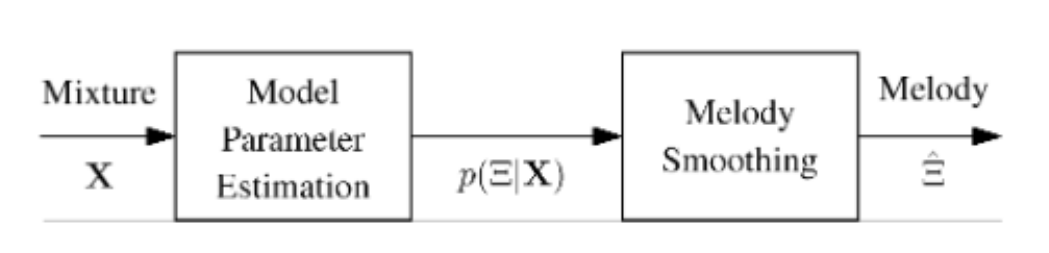
\includegraphics[scale=0.2]{images/fig1}
    \caption{System Outline}
    \label{fig:fig1}
\end{figure}

As shown in Fig. \ref{fig:fig1}, the overall system is a two step melody tracker which relies on parametrization of the power spectrogram. In the first step, parameters of a short time Fourier transform (STFT) of the mixture signal are estimated and the posterior probabilities are computed. The second step outputs the desired sequence after a melody smoothing block based on the Viterbi algorithm \cite{viterbi}.

\begin{figure}[H]
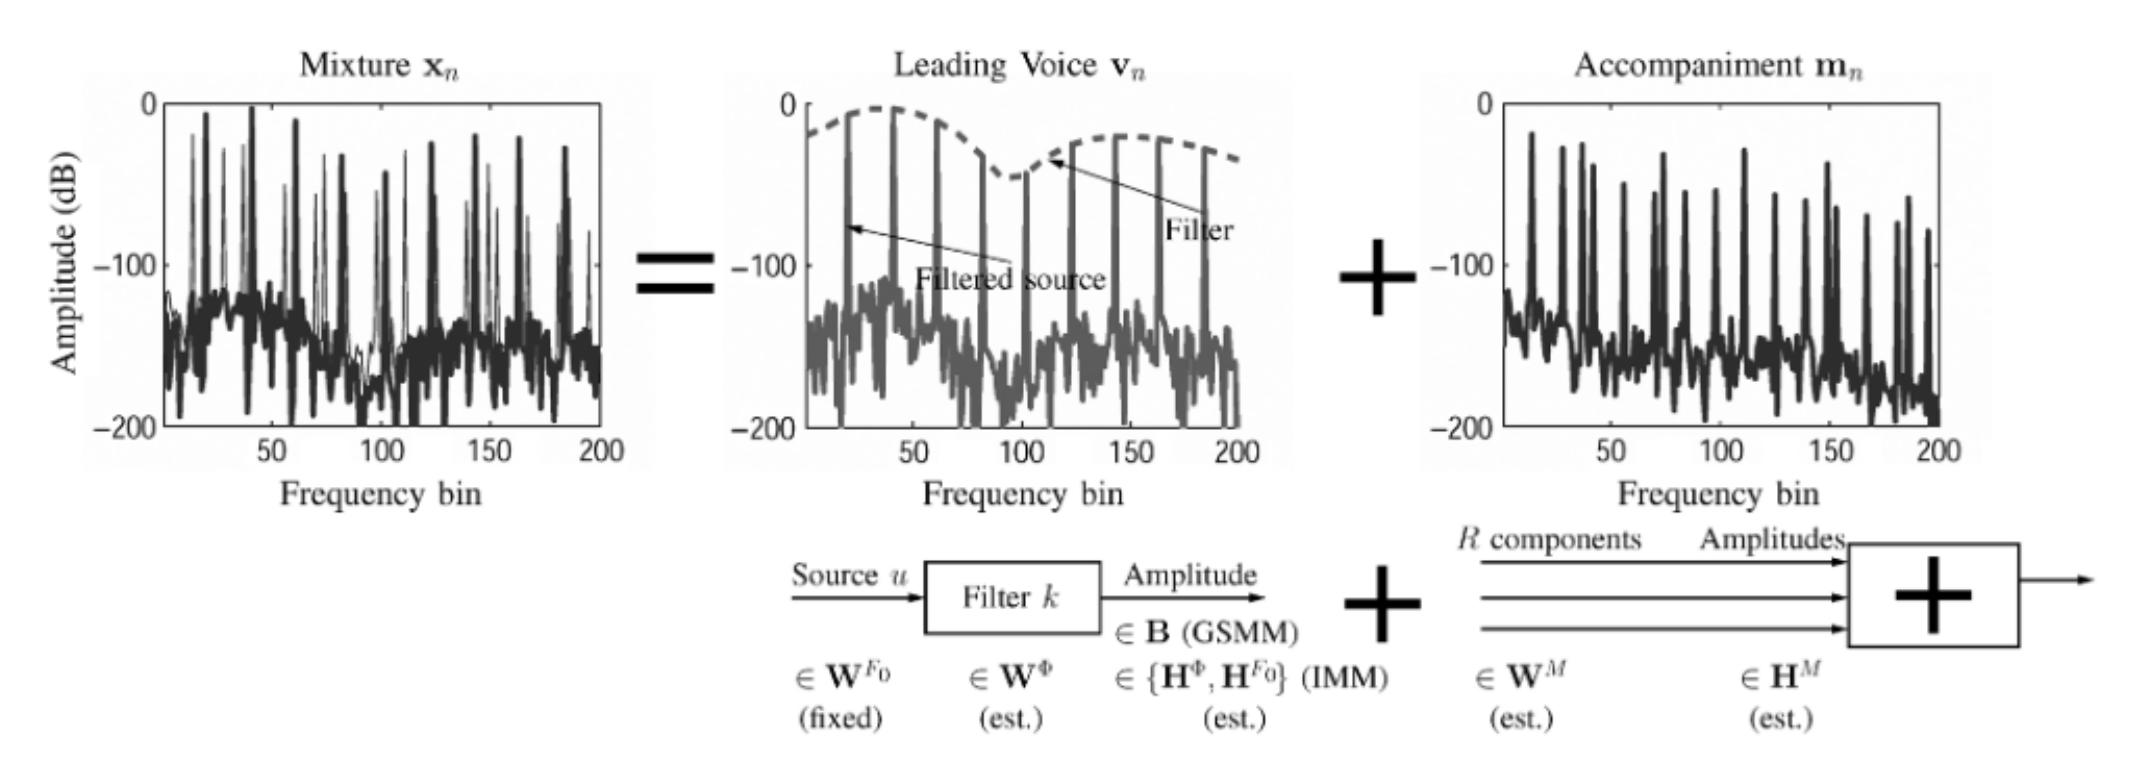
\includegraphics[scale=0.12]{images/fig2}
    \caption{Decomposition of frame into leading voice and accompaniment}
    \label{fig:fig2}
\end{figure}

Fig. \ref{fig:fig2} shows the general principle of the parametrization of the signal. A source filter model is fitted to the main melody part, to capture the variability of the lead voice in terms of pitch range and timbre; and the residual accompaniment, which consists of more stable pitch lines, is modelled in a non-negative matrix factorization (NMF) framework.

\begin{figure}[H]
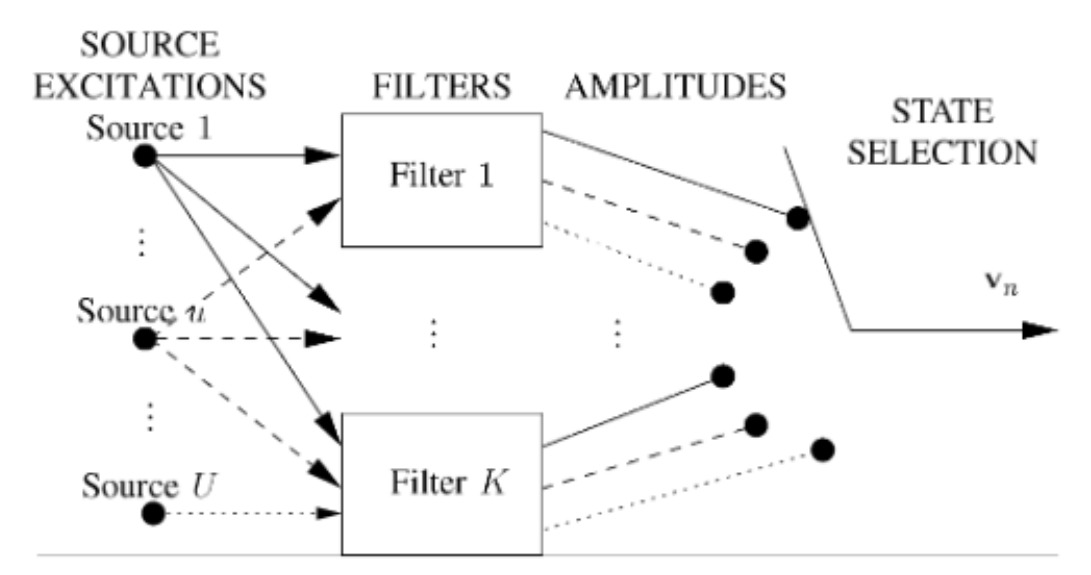
\includegraphics[scale=0.2]{images/fig3}
    \caption{Source/filter model}
    \label{fig:fig3}
\end{figure}

The source/filter model is depicted in \ref{fig:fig3}. Each source excitation is filtered through each of the filters and the amplitudes for a frame are applied to each of the output signals. The final state selector sets the active state for a given frame based on its likelihood given the source, filter pairs; and each of them is scaled by the amplitude. This likelihood estimation is similar to a Gaussian Mixture Model (GMM) and Expectation Maximization (EM) is deployed to solve for the parameters.

In practice, the number of filters and number of accompaniment components have been derived from testing different combinations, and remains fixed during evaluation.

\subsection{Feature Extraction}
\label{sec:features}
All the melody features have been derived from the fundamental frequencies (F0). For each of the 30 second audio track, F0 has been estimated at 5169 instances. The following features have been used:
\begin{itemize}
\item \textbf{Pitch Based}
		\begin{itemize}
		\item Mean F0
		\item Variance
		\item Max F0
		\item Min F0
		\item Skewness
		\item Kurtosis
		\end{itemize}
\item \textbf{Vibration based}
		\begin{itemize}
		\item Mean
		\item Variance
		\end{itemize}
\end{itemize}

Here, vibration has been calculated as the difference between consecutive recorded F0s.
Skewness is the measure of asymmetry data around the sample, and can be calculated as:
\begin{align}
s = \frac{E(x - \mu)^3}{\sigma^3}
\end{align}
Kurtosis is a measure of how outlier prone a distribution is, and can be calculated as:
\begin{align}
k = \frac{E(x - \mu)^4}{\sigma^4}
\end{align}

All the pitch based features were also considered incrementally for vibration based ones, however they hampered the accuracy, so they were dropped. Features related to the topology were also tested to the same result.

Features based on Mel Frequency Cepstrum Coefficients (MFCC) were used for a baseline comparison. Its mean and variance provided a total of 26 features, considering 13 coefficients. A combined feature set of the melody features and the MFCC ones was also used.

Melody features were calculated for both the original audio as well as the source extracted audio separately.

\subsection{Classification}
\label{classification}
Four different methods were used for classification:
\begin{itemize}
\item K-Nearest Neighbors (KNN) Classifier
\item Gaussian Naive Bayes (GaussianNB)
\item Support Vector Machine with linear kernel (linearSVC)
\item Support Vector machine with rbf kernel (SVC)
\end{itemize}

\subsection{Clustering}
\label{clustering}
K-Nearest Neighbors (KNN) algorithm was used for clustering. The accuracy score was calculated using the following measures:
\begin{itemize}
\item Homogeneity: each cluster contains only members of a single class \cite{cluster}
\item Completeness: all members of a given class are assigned to the same cluster.
\item V Measure: Harmonic mean of Homogeneity and Completeness.
\item Adjusted Rand Score: measures the similarity of the two assignments, ignoring permutations and with chance normalization.
\item Adjusted Mutual Info: measures the agreement of the two assignments, ignoring permutations.
\end{itemize}


\section{Implementation}
The following tools were used for carrying out the above mentioned tasks:
\begin{itemize}
\item \textbf{separateLeadStereo} from the pyFASST package \cite{durrieu03} was used for source separation. pyFASST is a python implementation of the flexible Audio Source Separation Toolbox. The dataset used provided mono 16-bit audio files, so the code which was primarily for stereo had to be adapted a bit to suit the dataset.
\item \textbf{Scikit Learn} has been used for implementing all the classification and clustering tasks. The classifiers have been used with their default configurations.
\item \textbf{MFCC} implementation from Auditory Toolbox \cite{auditoryToolbox}  is used for calculating the MFCC features.
\item All the intermediate scripts for processing have been written in python and matlab. Python libraries scipy and numpy were used for all the calculations.
\end{itemize}

\section{Dataset}
A subset of the GTZAN dataset \cite{gtzan} is used for all the evaluation criteria. The dataset consists of 1000 audio tracks each 30 seconds long. It contains 10 genres, each represented by 100 tracks. The tracks are all 22050Hz Mono 16-bit audio files in .au format. Of these the first 10 audio tracks from each of the 10 genres have been analyzed. The audio files had to be converted from .au format to the .wav format for further processing. A linux utility known as soxexam was used for the conversion.

The dataset contains tracks under the following categories (the description is from their respective Wikipedia articles):
\begin{itemize}
\item \textbf{Blues}: Cyclic musical form in which a repeating progression of chords mirrors the call and response scheme commonly found in African and African-American music \cite{blues}
\item \textbf{Classical}: Classical music has been noted for its development of highly sophisticated forms of instrumental music \cite{classical}
\item \textbf{Country}: Country music often consists of ballads and dance tunes with generally simple forms and harmonies accompanied by mostly string instruments \cite{country}
\item \textbf{Disco}: Includes a large pop band, with several chordal instruments \cite{disco}
\item \textbf{Hiphop}: Consists of a stylized rhythmic music that commonly accompanies rapping \cite{hiphop}
\item \textbf{Jazz}: Includes qualities such as swing, improvising, group interaction, developing an individual voice, and being open to different musical possibilities \cite{jazz}
\item \textbf{Metal}: A thick, massive sound, characterized by highly amplified distortion, extended guitar solos, emphatic beats, and overall loudness. \cite{metal}
\item \textbf{Pop}: Includes common employment of repeated choruses, melodic tunes, and catchy hooks. \cite{pop}
\item \textbf{Reggae}: It incorporates some of the musical elements of rhythm and blues \cite{reggae}
\item \textbf{Rock}: It has centered on the electric guitar, usually as part of a rock group with electric bass guitar and drums.\cite{rock}
\end{itemize}

While the minute details of each of the music form is not of particular interest for this project, the point to take away is that there is a lot of overlap in between these music forms, which makes it difficult to pin down some of the audio tracks to a specific genre. Indeed the boundaries for the different genres is also very fine. In fact, an audio track could very well in reality belong to two or more genres. Though the dataset has been used by many researchers for genre classification, there are still errors in classifying the audio tracks, which has been looked into by \cite{sturm}.

\section{Results}

The first set of observations has been done on the complete set of genres; whereas for the next set, we narrow down to classical, pop and rock genres, as their main melody is well suited for the feature set we are trying to capture.

Classification and clustering tasks (mentioned in section \ref{classification} and \ref{clustering}) have been performed on features extracted as explained in section \ref{sec:features}. For classification, a 50:50 split for training and testing was used. Clustering was performed using all the  audio tracks.

\begin{table}[H]
	\centering
    \begin{tabular}{| p{1.85cm} | l | p{1.8cm} | p{1.5cm} | l |}
    \hline
    \textbf{Classification} & \textbf{KNN} & \textbf{Gaussian Naive Bayes} & \textbf{Linear SVC} & \textbf{SVC} \\ \hline
    \textbf{MFCC} & \textbf{0.32} & 0.52 & \textbf{0.6} & \textbf{0.44} \\ \hline
    \textbf{Pitch Solo} & 0.28 & 0.36 & 0.22 & 0.22 \\ \hline
    \textbf{Pitch Orig} & 0.22 & 0.3 & 0.28 & 0.2 \\ \hline
    \textbf{Combined Solo} & 0.28 & \textbf{0.54} & 0.16 & 0.26 \\ \hline
    \textbf{Combined Orig} & 0.22 & 0.3 & 0.1 & 0.2 \\
    \hline
    \end{tabular}
    \caption{Classification Accuracy considering all genres}
    \label{table:classAll}
\end{table}

\begin{table}[H]
	\centering
	\resizebox{\columnwidth}{!}{%
    \begin{tabular}{| p{1.1cm} | l | l | p{1cm} | p{1cm} | p{1cm} |}
    \hline
    \textbf{Clustering} & \textbf{Homogeneity} & \textbf{Completeness} & \textbf{V Measure} & \textbf{Adjusted Rand Score} & \textbf{Adjusted Mutual Info} \\ \hline
    \textbf{MFCC} & \textbf{0.411} & \textbf{0.437} & \textbf{0.424} & \textbf{0.173} & \textbf{0.262}\\ \hline
    \textbf{Pitch Solo} & 0.379 & 0.418 & 0.397 & 0.160 & 0.234 \\ \hline
    \textbf{Pitch Orig} & 0.343 & 0.412 & 0.374 & 0.122 & 0.203\\ \hline
    \textbf{Combined Solo} & 0.372 & 0.416 & 0.393 & 0.134 & 0.228\\ \hline
    \textbf{Combined Orig} & 0.350 & 0.401 & 0.374 & 0.128 & 0.207 \\
    \hline
    \end{tabular}
    }
    \caption{Clustering Score considering all genres}
    \label{table:clusterAll}
\end{table}

Table \ref{table:classAll} and \ref{table:clusterAll} show the accuracies for classification and clustering respectively while considering all the genres. We see that our set of features perform very poorly in general for most cases, even when compared to the MFCC baseline. However, we do see some trends, the pitch features extracted from the source separated audio are performing better than those extracted from the original audio.

\begin{table}[H]
	\centering
    \begin{tabular}{| p{1.85cm} | l | p{1.8cm} | p{1.5cm} | l |}
    \hline
    \textbf{Classification} & \textbf{KNN} & \textbf{Gaussian Naive Bayes} & \textbf{Linear SVC} & \textbf{SVC} \\ \hline
    \textbf{MFCC} & 0.46 & 0.73 & 0.93 & 0.6 \\ \hline
    \textbf{Pitch Solo} & 0.46 & 1.00 & 0.93 & 0.8 \\ \hline
    \textbf{Pitch Orig} & 0.46 & 0.93 & 1.00 & 0.6 \\ \hline
    \textbf{Combined Solo} & 0.46 & 0.93 & 0.93 & 0.8\\ \hline
    \textbf{Combined Orig} & 0.46 & 0.86 & 1.00 & 0.6 \\
    \hline
    \end{tabular}
    \caption{Classification Accuracy for specific genres}
    \label{table:classReduced}
\end{table}

\begin{table}[H]
	\centering
	\resizebox{\columnwidth}{!}{%
    \begin{tabular}{| p{1.1cm} | l | l | p{1cm} | p{1cm} | p{1cm} |}
    \hline
    \textbf{Clustering} & \textbf{Homogeneity} & \textbf{Completeness} & \textbf{V Measure} & \textbf{Adjusted Rand Score} & \textbf{Adjusted Mutual Info} \\ \hline
    \textbf{MFCC} & 0.389 & 0.441 & 0.413 & 0.340 & 0.342 \\ \hline
    \textbf{Pitch Solo} & 1.00 & 1.00 & 1.00 & 1.00 & 1.00\\ \hline
    \textbf{Pitch Orig} & 1.00 & 1.00 & 1.00 & 1.00 & 1.00\\ \hline
    \textbf{Combined Solo} & 1.00 & 1.00 & 1.00 & 1.00 & 1.00\\ \hline
    \textbf{Combined Orig} & 1.00 & 1.00 & 1.00 & 1.00 & 1.00 \\
    \hline
    \end{tabular}
    }
    \caption{Clustering Score for specific genres}
    \label{table:clusterReduced}
\end{table}

Tables \ref{table:classReduced} and \ref{table:clusterReduced} cut down to only the classical, pop and rock genres. This is when we can actually see the power of our feature set. In both the cases, the pitch features are performing way better than MFCC, achieving perfect scores for clustering, and near perfect classification too. The MFCC feature set when combined with pitch features also provides promising results. 

In some more experiments which have not been published here, the accuracy did not have a gradual drop as the number of genres were increased. However, it depended on which particular genre was taken into consideration. Certain genres lead to a rapid deterioration while some did not lead to much of a decline.

\section{Conclusion}

The above results show that the feature set is highly dependent on genres taken into account. Indeed, previous work on using solely pitch features \cite{salamon01} used a synthetic dataset which was suited to the melody features. Thus, though it is highly unlikely that the features be used in isolation, augmenting them to already used features can result in improvements as shown with the MFCC example. Also, using the features extracted from source separated audio provides a more stable prediction as compared to those from the    original audio itself.

\section{Future Work}

Combining the melody related features with the existing state of the art and analysing the performance is something which should shed more of light on the dependability of these features. More complex features could be derived from the fundamental frequencies or from the pitch contours in general, which was not explored in detail in this paper.

% trigger a \newpage just before the given reference
% number - used to balance the columns on the last page
% adjust value as needed - may need to be readjusted if
% the document is modified later
%\IEEEtriggeratref{8}
% The "triggered" command can be changed if desired:
%\IEEEtriggercmd{\enlargethispage{-5in}}

% references section

% can use a bibliography generated by BibTeX as a .bbl file
% BibTeX documentation can be easily obtained at:
% http://www.ctan.org/tex-archive/biblio/bibtex/contrib/doc/
% The IEEEtran BibTeX style support page is at:
% http://www.michaelshell.org/tex/ieeetran/bibtex/
%\bibliographystyle{IEEEtran}
% argument is your BibTeX string definitions and bibliography database(s)
%\bibliography{IEEEabrv,../bib/paper}
%
% <OR> manually copy in the resultant .bbl file
% set second argument of \begin to the number of references
% (used to reserve space for the reference number labels box)
\begin{thebibliography}{100}

\bibitem{scaringella}
N.~Scaringella, G.~Zoia, and D.~Mlynek, "Automatic genre classification of music content: A survey," IEEE Signal Process. Mag., vol. 23, no. 2, Mar. 2006
\bibitem{durrieu01}
J.L.~Durrieu, G.~Richard, B.~Davis, C.~Fevotte, "Source/Filter Model for Unsupervised Main Melody Extraction From Polyphonic Audio Signals," IEEE Transactions on Audio, Speech, and Language Processing, vol. 18, no. 3, Mar. 2010
\bibitem{durrieu02}
J.L.~Durrieu, G.~Richard, B.~Davis, "A Musically Motivated Mid-Level Representation for Pitch Estimation and Musical Audio Source Separation," IEEE Journal of Selected Topics in Signal Processing, vol. 5, no. 6, Oct. 2011
\bibitem{salamon01}
J.~Salamon, E.~Gomez, B.~Rocha, "Musical Genre Classifcation using Melody Features extracted from Polyphonic Music Signals"
\bibitem{durrieu03}
http://www.durrieu.ch/research/jstsp2010.html
\bibitem{gtzan}
http://marsyas.info/download/data\_sets/
\bibitem{blues}
http://en.wikipedia.org/wiki/Blues
\bibitem{classical}
http://en.wikipedia.org/wiki/Classical\_music
\bibitem{country}
http://en.wikipedia.org/wiki/Country\_music
\bibitem{disco}
http://en.wikipedia.org/wiki/Disco
\bibitem{hiphop}
http://en.wikipedia.org/wiki/Hip\_hop\_music
\bibitem{jazz}
http://en.wikipedia.org/wiki/Jazz
\bibitem{metal}
http://en.wikipedia.org/wiki/Heavy\_metal\_music
\bibitem{pop}
http://en.wikipedia.org/wiki/Pop\_music
\bibitem{reggae}
http://en.wikipedia.org/wiki/Reggae
\bibitem{rock}
http://en.wikipedia.org/wiki/Rock\_music
\bibitem{sturm}
Sturm, Bob L. "An analysis of the GTZAN music genre dataset." Proceedings of the second international ACM workshop on Music information retrieval with user-centered and multimodal strategies. ACM, 2012.
\bibitem{auditoryToolbox}
Slaney, Malcolm. "Auditory toolbox." Interval Research Corporation, Tech. Rep 10 (1998): 1998.
\bibitem{peeters}
Peeters, Geoffroy. "{A large set of audio features for sound description (similarity and classification) in the CUIDADO project}." (2004).
\bibitem{panagakis}
Panagakis, Yannis, Constantine Kotropoulos, and Gonzalo R. Arce. "Music genre classification via sparse representations of auditory temporal modulations." Proc. European Signal Process. Conf., Glasgow, Scotland. 2009.
\bibitem{cluster}
Rosenberg, Andrew, and Julia Hirschberg. "V-Measure: A Conditional Entropy-Based External Cluster Evaluation Measure." EMNLP-CoNLL. Vol. 7. 2007.
\bibitem{viterbi}
Forney Jr, G. David. "The viterbi algorithm." Proceedings of the IEEE 61.3 (1973): 268-278.

\end{thebibliography}

% biography section
% 
% If you have an EPS/PDF photo (graphicx package needed) extra braces are
% needed around the contents of the optional argument to biography to prevent
% the LaTeX parser from getting confused when it sees the complicated
% \includegraphics command within an optional argument. (You could create
% your own custom macro containing the \includegraphics command to make things
% simpler here.)
%\begin{biography}[{\includegraphics[width=1in,height=1.25in,clip,keepaspectratio]{mshell}}]{Michael Shell}
% or if you just want to reserve a space for a photo:



% that's all folks
\end{document}


